\documentclass[book.tex]{subfiles}
\begin{document}
\section{Source Code}
The game engine was released on July 21, 1995. 20 years later it is still there on the company ftp\footnote{Transfer File Protocol (along with Finger where J.C.Carmack used to blog) was commonly used in the 90s in the blessed time where you did not have to encrypt everything on the wire.}:\\ 
\\\codeword{ftp://ftp.idsoftware.com/idstuff/source/wolfsrc.zip}.\\
\\
\textbf{\underline{Trivia :}} Before the times of nmap and WireShark, ftp was commonly used to transfer files: It was simple and naively transmitted username and password in clear. Needless to say it did not age well...\\

\section{First Contact}
\section{PG13}
The file \codeword{woldsrc.zip} contains an other self-extracting PKZIP archive. It was a convenience back in the day but it is not practical nowadays. You can deflate it with:\\
\\\codeword{unzip WOLFSRC.1}.\\
\\The source code actually contains more than just \codeword{.H} (headers) and \codeword{.C} (code) files. Also present are:
\begin{itemize}
\item \codeword{.EQU}
\item \codeword{\_WL1.H}
\item \codeword{\_WL6.H}
\item \codeword{\_SOD.H}
\item \codeword{\_SDM.H}
\item \codeword{GOODSTUF.TXT} A letter from a POW playing Wolfenstein 3D.
\item \codeword{.ASM} Assembly optimized routines. Also contains  routines to access VGA and refresh screen.
\item \codeword{SIGNON.OBJ/}: The startup screen showing the system characteristic (RAM, EMS, XMS, Joystick, SoundCards) was linked in the binary. Because that screen was showed before any sub-system was started. TODO: This should be a trivia.
\item \codeword{GAMEPAL.OBJ/} Game palette. Hardcoded and linked in the executable for the same reason described previously.
\item \codeword{README/} How to build. You can find a complete tutorial in the Annexe of this book.
\item \codeword{RULES.ASI} ???
\item \codeword{SV.EXE} ???
\item Many files resulting in a previous compilation attempt.
\end{itemize}
A quick stats:\\
\begin{verbatim}
wolfsrc\$ cloc-1.64.pl .

      96 text files.
      94 unique files.                              
      27 files ignored.

--------------------------------------------------------------------------
Language                files          blank        comment           code
--------------------------------------------------------------------------
C++                        26           5750           6201          21169
C/C++ Header               42            802            660           3900
Assembly                   10            669            732           2150
DOS Batch                   1              1              0              4
--------------------------------------------------------------------------
SUM:                       79           7222           7593          27223
--------------------------------------------------------------------------
\end{verbatim}
The game engine is mostly C with a few ASM routines for optimized stuff and I/O.\\


 \begin{fancyquotes}
   We didn't have spell checkers in our editors back then, and I always had poor spelling.  The word "collumn" appears in the source code dozens of times.  After I released the source code, one of the emails that stands out in memory read:
 \bigskip \\
It's "COLUMN", you dumb @\#\$\% !\\
 \bigskip \\
\textbf{John Carmack - Programmer}
 \end{fancyquotes}

\begin{fancyquotes}
Estimated completion time ?  
\textbf{John Carmack - Programmer}
 \end{fancyquotes}
 
\section{Architecture}

The engine is made of sub-systems called Managers:
\begin{itemize}
	\item Memory
	\item Page
	\item Video
	\item Cache
	\item Sound
	\item User
	\item Input
\end{itemize}
Together they harness the machine to play sound, music and display the two phases of the game:
\begin{itemize}
	\item 2D Menus
	\item 3D Action
\end{itemize}


\begin{figure}[H]
\centering
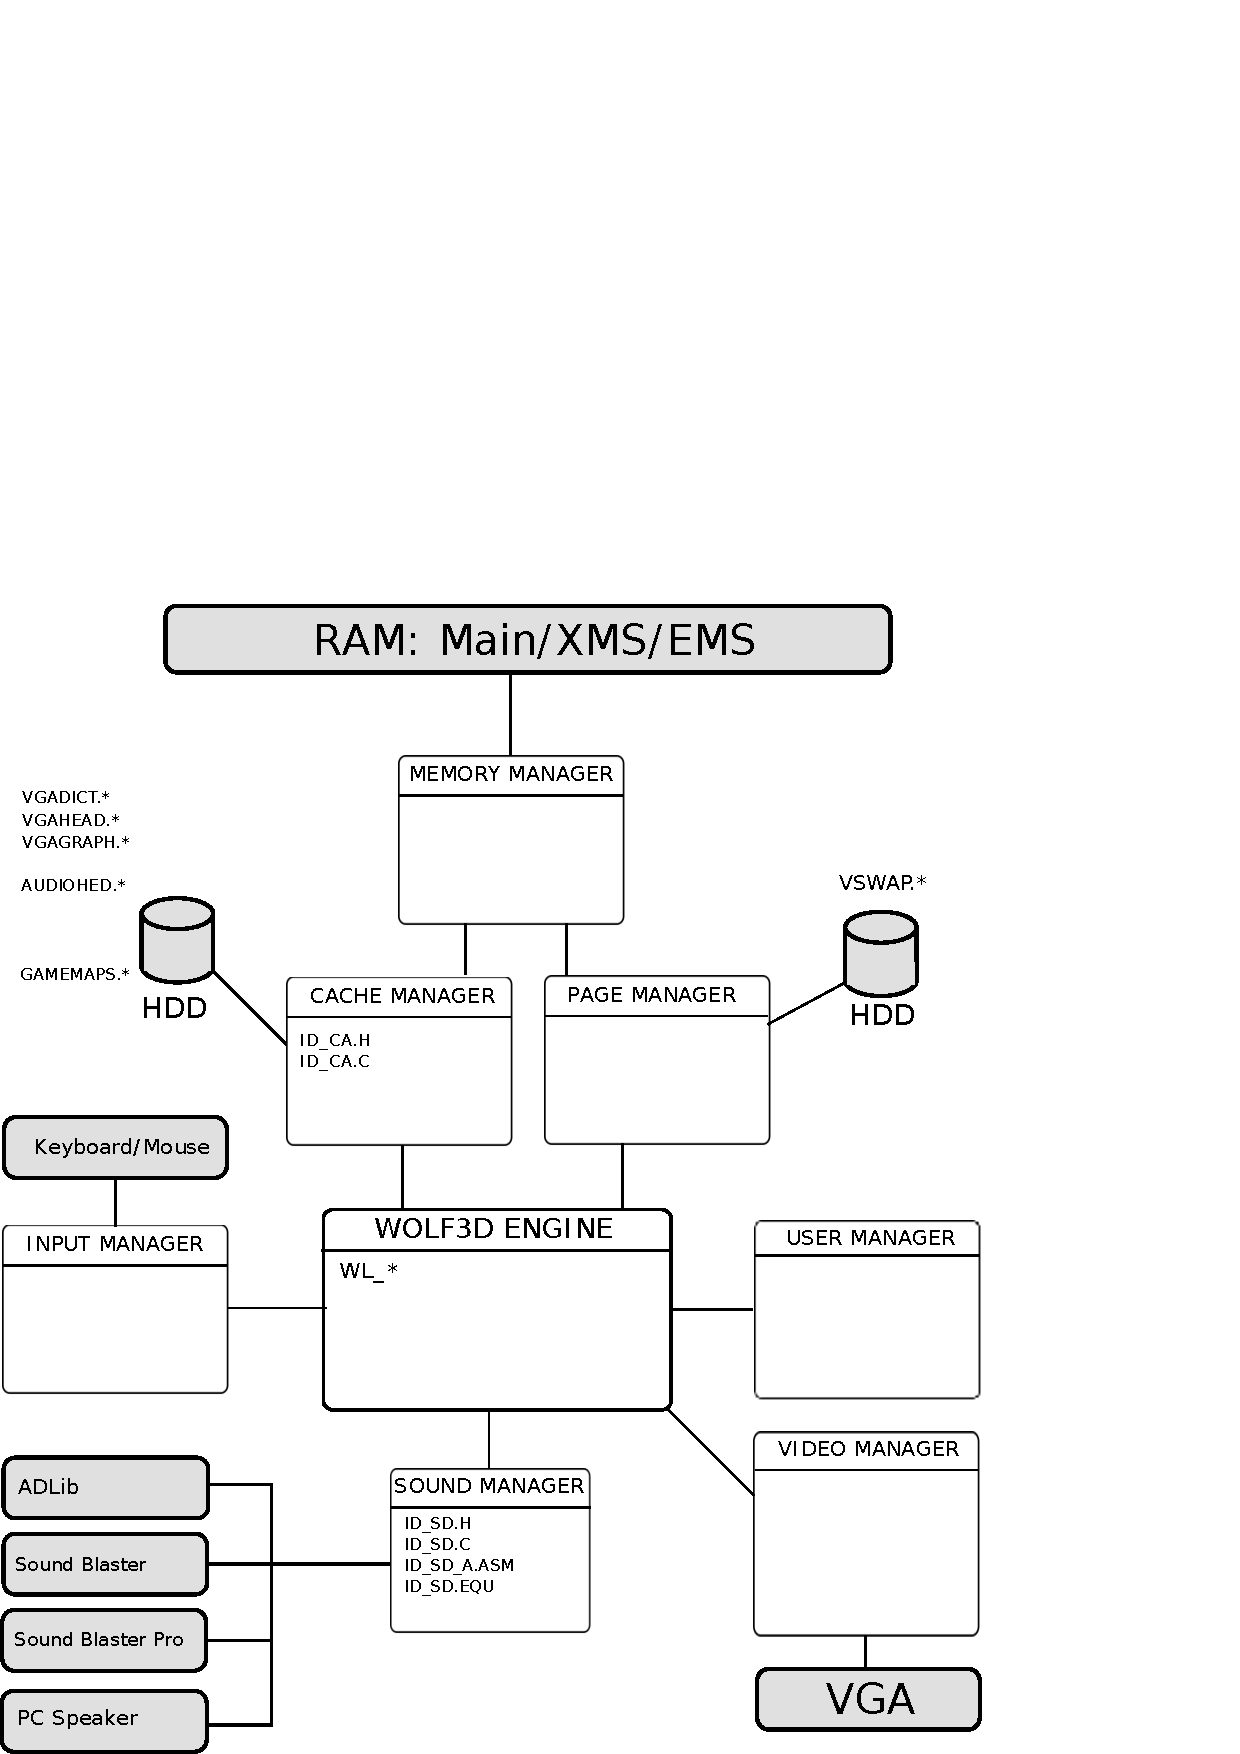
\includegraphics[width=\textwidth]{imgs/architecture.pdf}
\caption{Architecture and sub-systems.}
\label{fig:architecture}
\end{figure}


\subsection{Memory Manager (MM)}

\subsection{Page Manager (PM)}

The Page Manager harness the three types of RAM available: Conventional, XMS and XML. It abstract this complexity behind a Paging system.\\
Is it where the loading screen shows a progress bar ?
"Get Psyched !!!": Fill up the cache ?
Trivia: The progress bar was called a "thermometer".
The Page Manager provides all asset during 3D rendition. 
It loads as many "Pages" as possible in Main, XMS and EMS memory during the get Psyched screen.
TODO: Add a screenshot.
It uses a Least Frequency Used eviction policy if not all asset fit in RAM. VSWAP.WL6 is 1.6MB -> Recommended configuration 2MB RAM..but the game would run with just 640KB.
\subsection{Video Manager (VW)}


\subsection{Cache Manager (CA)}
The Cache Manager takes care of all the assets during Menu Phases: Sprites, Music, Sounds.
\subsection{Sound Manager (SD)}
The Sound Manager abstract interaction with all four sound systems supported: PC Speaker, ADLib (Music only), Sound Blaster (Mono), Sound Blaster Pro (Stereo).
\subsection{User Manager (US)}


\subsection{Input Manager (IN)}
Abstract interaction with keyboard and mouse.

\end{document}